\chapter{中央データベースとローカルデータベースのデータ同期ツールに関する研究}

開発した機能が生産時に十分であるかどうか見積もりは今後の開発を効率よく進めていく上で重要である。
生産時のデータの数や量を想定してその際のシステム性能を見積もることで、今の実装で十分かどうか、改善が必要な場合どのように改善すればいいかを知ることができる。
中央データベースとローカルデータベースのデータ同期機能に関して処理時間評価を行った。
詳細について以下で説明する。

\section{サーバーの設置場所による処理時間の違い}
4章で述べたように、中央データベースはチェコに設置されている。
そのため試験結果のアップロードに関して、各組み立て機関から接続しデータ送信する処理時間は、機関の場所に大きく依存すると考えられる。
世界的にデータ同期ツールが不自由なく動くことに向けた開発、改善に役立てることを目的として、データを送信する処理時間を、以下の3つの場所に置かれているサーバーを用いて測定した。

\begin{itemize}
  \item 日本、高エネルギー加速器研究所(KEK) 
  \item アメリカ、バークレー研究所(LBL)
  \item スイス、欧州原子核研究機構(CERN)
\end{itemize}

各サーバーの性能を表\ref{server_spec}に示す。また各サーバーが置かれている場所の位置関係を図\ref{server_geometry}に示す。

\begin{table}[tbp]
\caption[サーバーの性能一覧]{サーバーの性能一覧}
\label{server_spec}
\scalebox{0.9}{
  \begin{tabular}{|l|llll|l|l|} \hline
    設置機関 & CPU & & & & Memory & Disk \\
     & Type & Core & Thread & Clock speed[GHz]& [kB] & [GB] \\ \hline 
    KEK & Intel(R) Core(TM) i7-6700 & 4 & 8 & 3.4 & 15,981,000 & 197\\
    LBL & Intel(R) Core(TM) i7-8700 & 6 & 12 & 3.7 & 32,628,000 & 233\\
    CERN & Intel Core Processor (Broadwell, IBRS) & 1 & 10 & 2.2 & 29,978,888 & 80\\ \hline
  \end{tabular}
}
\end{table}


\begin{figure}[bpt]\centering
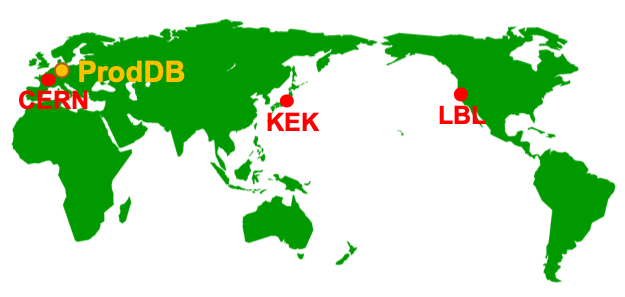
\includegraphics[width=10cm]{server_geometry}
\caption[各サーバの位置関係]{各サーバの位置関係}
\label{server_geometry}
\end{figure}

これらのサーバーは実際に生産の際に使用するものと同程度の性能を持ち、サーバーが置かれている環境も生産時と同じであるとしている。
回線の混雑具合などによる処理時間の低下は、本測定では考慮に入れていない。

\subsection{データ同期ツールに使用するAPI}
中央データベースのデータ取得には、用意されているAPIのサービスを使用している。
ローカルデータベースとのデータ同期ツールの中で主に使用しているAPIを表\ref{pd_API}に示す。

\begin{table}[tbp]
  \begin{center}
  \caption[データ同期ツールの中で使用しているAPI]{データ同期ツールの中で使用したAPI}
  \label{pd_API}
  \scalebox{0.7}{
    \begin{tabular}{|lll|} \hline
      関数名 & 処理の内容 & 本ツールでの使用用途\\ \hline
      getComponent            & 
      登録した装置情報の取得 & 主にダウンロード時におけるモジュールやチップの情報取得に用いる。\\
      uploadTestRunResults    & 
      テスト結果生成 & 読み出し試験結果生成の際に用いる。 \\
      createTestRunAttachment & 
      あるテスト結果に対するバイナリファイルの添付 & 読み出し試験結果生成後にファイルを添付する際に用いる。\\ \hline
    \end{tabular}
  }
  \end{center}
\end{table}

\subsection{API使用にかかる時間}
上述したAPI使用時の処理時間を各サーバーで測定した。
以下の3つの測定を行なった。
\begin{itemize}
  \item getComponentを用いた、登録モジュール情報1つの取得時間測定
  \item createTestRunAttachmentを用いて、ある試験結果ページに1Byteのデータファイルを添付する時間測定
  \item createTestRunAttachmentを用いて、ある試験結果ページに容量の異なるデータファイルを添付、容量に対する時間依存性を測定
\end{itemize}

最初の2項目に関して、各処理時間についてまとめたものを表\ref{getting_1module}、\ref{sendpd_1byte}に示す。
またファイル容量と処理時間の関係を図\ref{datasize_vs_time}に示す。1Byteでの測定点も含んでいる。

\begin{table}[tbp]
  \begin{minipage}[t]{.45\textwidth}
  \begin{center}
  \caption[モジュール情報の取得にかかる時間]{モジュール情報の取得にかかる時間}
  \label{getting_1module}
    \begin{tabular}{|ll|} \hline
      サーバー & 処理時間[秒] \\ \hline
      KEK & 0.49 $\pm$ 0.02 \\ 
      LBL & 0.37 $\pm$ 0.02 \\ 
      CERN & 0.30 $\pm$ 0.04 \\ \hline 
    \end{tabular}
  \end{center}
  \end{minipage}
  \hfill 
  \begin{minipage}[t]{.45\textwidth}
  \begin{center}
  \caption[1Byteのデータファイル添付にかかる処理時間]{1Byteのデータファイル添付にかかる処理時間}
  \label{sendpd_1byte}
    \begin{tabular}{|ll|} \hline
      サーバー & 処理時間[秒] \\ \hline
      KEK & 0.54 $\pm$ 0.04 \\ 
      LBL & 0.34 $\pm$ 0.03 \\ 
      CERN & 0.39 $\pm$ 0.02 \\ \hline 
    \end{tabular}
  \end{center}
  \end{minipage}
\end{table}

\begin{figure}[bpt]\centering
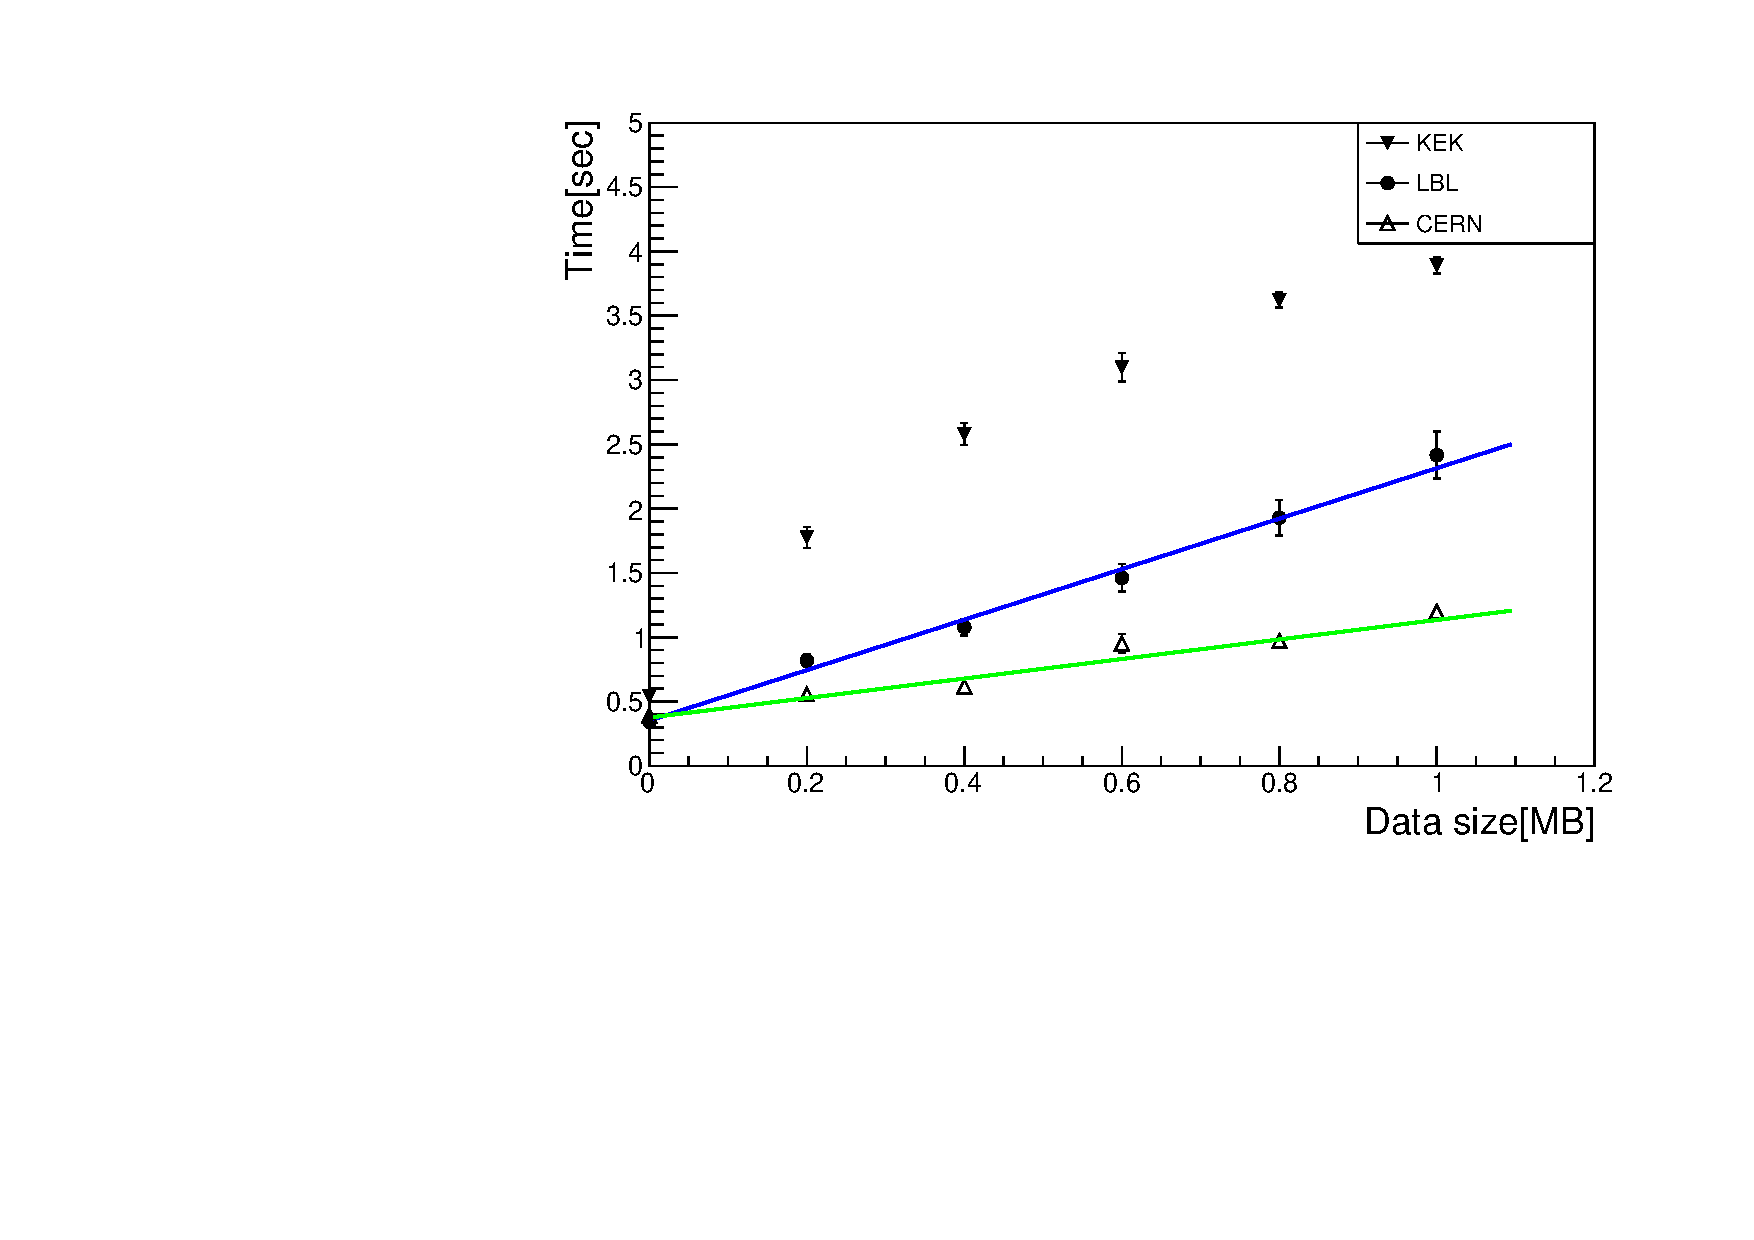
\includegraphics[width=7cm,angle=270]{datasize_vs_time.pdf}
\caption[添付するファイルサイズと処理時間の関係]{添付するファイルサイズと処理時間の関係}
\label{datasize_vs_time}
\end{figure}

\section{モジュールIDのダウンロード機能確認と処理時間測定}
\subsection{アルゴリズム}
開発したモジュールIDをダウンロードするツールのアルゴリズムについて記す。
アルゴリズムのイメージを図\ref{download_algorithm}に示す。

\begin{figure}[bpt]\centering

\includegraphics[width=1cm]{figure}
\caption[ダウンロードアルゴリズムのイメージ図]{ダウンロードアルゴリズムのイメージ図}
\label{download_algorithm}
\end{figure}

\subsection{機能確認}
KEKで組み立てられた6台のモジュールを中央データベースに登録し、ダウンロードを行った。
登録したモジュールを表\ref{registered_kek_module}、ダウンロードをしてアプリケーションで確認した様子を図\ref{registered_kek_module_viewer}に示す。

\begin{table}[tbp]
\begin{center}
\caption[登録したKEKモジュール]{登録したKEKモジュール}
\label{registered_kek_module}
  \begin{tabular}{|ll|} \hline
    1 & 2 \\ \hline
    result 1 & result 2 \\ \hline 
  \end{tabular}
\end{center}
\end{table}

\begin{figure}[bpt]\centering

\includegraphics[width=1cm]{figure}
\caption[ダウンロードしたKEKモジュールがアプリケーションで確認できている様子]{ダウンロードしたKEKモジュールがアプリケーションで確認できている様子}
\label{registered_kek_module_viewer}
\end{figure}

\subsection{処理時間測定}
KEKモジュールをダウンロードした際の処理時間を測定した。
これについてまとめたものを表\ref{download_measurement}に示す。

\begin{table}[tbp]
\begin{center}
\caption[ダウンロード処理時間測定]{ダウンロード処理時間測定}
\label{download_measurement}
  \begin{tabular}{|ll|} \hline
    1 & 2 \\ \hline
    result 1 & result 2 \\ \hline 
  \end{tabular}
\end{center}
\end{table}

\subsection{改善点}

\section{読み出し試験結果のアップロード機能確認と処理時間測定}
\subsection{アルゴリズム}
読み出し試験の結果をアップロードするツールのアルゴリズムについて記す。
アルゴリズムのイメージを図\ref{upload_algorithm}に示す。

\begin{figure}[bpt]\centering

\includegraphics[width=1cm]{figure}
\caption[アップロードアルゴリズムのイメージ図]{アップロードアルゴリズムのイメージ図}
\label{download_algorithm}
\end{figure}

\subsection{機能確認}
5章でアップロード機能については確認したため、ここでは割愛する。

\subsection{処理時間測定}
5章で行った読み出し試験の結果を中央データベースにアップロードした際の処理時間測定を行った。
これについてまとめたものを表\ref{upload_measurement}に示す。

\begin{table}[tbp]
\begin{center}
\caption[アップロード処理時間測定]{アップロード処理時間測定}
\label{upload_measurement}
  \begin{tabular}{|ll|} \hline
    1 & 2 \\ \hline
    result 1 & result 2 \\ \hline 
  \end{tabular}
\end{center}
\end{table}

\subsection{改善点}
構造を変えることかなあ。
